% answers.tex —— 2017 年·全国Ⅰ卷·理科 · 参考答案与详细解析片段
% 由 tools/generate_projects.py 依来源总账自 2017/2017_数学真题_理_试题.md + 2017/2017_数学真题_理_解析正文.md + 2017/2017_数学真题_理_答案要点.md 生成，勿手改（改源 MD 后重跑）


\begin{gknotice}
\textbf{ 解析归属声明}：本文解析由本库编写者根据试题\textbf{独立推导}，\textbf{非官方标准答案}。若与官方发布版本不一致，以官方为准。

\textbf{ 卷种提示}：本卷为文理分科时代的旧结构，含\textbf{现已取消}的选做题（第 22/23 题）与\textbf{已删除}的三视图（第 7 题）、程序框图（第 8 题）考点。
\end{gknotice}

\par\medskip

\gkpart{一、选择题}

\begin{answer}
\gksolhead{1}{集合运算}

\textbf{题目}：

已知集合 $A=\{x\mid x<1\}$，$B=\left\{x\mid3^{x}<1\right\}$，则\mbox{（　　）}

\begin{gkopts}(2)
\task A．$A\cap B=\{x\mid x<0\}$
\task B．$A\cup B=\mathbf R$
\task C．$A\cup B=\{x\mid x>1\}$
\task D．$A\cap B=\varnothing$
\end{gkopts}

\Needspace{4\baselineskip}
\textbf{解析}

\Needspace{5\baselineskip}
先化简 $B$。指数函数 $y=3^{x}$ 单调递增，$3^{x}<1=3^{0}$ 等价于

\nopagebreak[4]
\[x<0\]

即 $B=\{x\mid x<0\}$。

\Needspace{5\baselineskip}
显然 $B\subseteq A$（$x<0$ 必然 $x<1$），于是

\nopagebreak[4]
\[A\cap B=B=\{x\mid x<0\},\qquad A\cup B=A=\{x\mid x<1\}\]

逐项核对：A ；B （并集是 $x<1$，不是 $\mathbf R$）；C ；D 。

\gkanswer{答案：A（$A\cap B=\{x\mid x<0\}$）}

\par\medskip

\end{answer}
\begin{answer}
\gksolhead{2}{几何概型 · 太极图}

\textbf{题目}：

如图，正方形 $ABCD$ 内的图形来自中国古代的太极图，正方形内切圆中的黑色部分和白色部分关于正方形的中心成中心对称。在正方形内随机取一点，则此点取自黑色部分的概率是\mbox{（　　）}
\nopagebreak[4]
\begin{center}% 2017 全国Ⅰ卷 理2/文4：正方形内的太极图（黑白关于中心成中心对称）
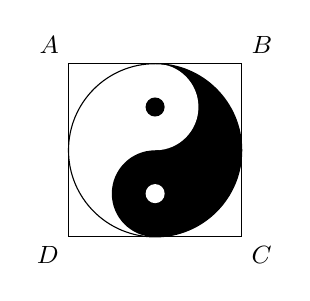
\begin{tikzpicture}[scale=1.1, font=\small]
  % 正方形 ABCD（A 左上、B 右上、C 右下、D 左下），边长 2，内切圆半径 1
  \draw (-1,-1) rectangle (1,1);
  \node[above left]  at (-1, 1) {$A$};
  \node[above right] at ( 1, 1) {$B$};
  \node[below right] at ( 1,-1) {$C$};
  \node[below left]  at (-1,-1) {$D$};
  \begin{scope}
    \clip (0,0) circle (1);
    % 右半黑
    \fill[black] (0,1) arc (90:-90:1) -- cycle;
    % 上小圆白、下小圆黑，构成 S 形分界
    \fill[white] (0,0.5) circle (0.5);
    \fill[black] (0,-0.5) circle (0.5);
    % 鱼眼
    \fill[black] (0,0.5) circle (0.11);
    \fill[white] (0,-0.5) circle (0.11);
  \end{scope}
  \draw (0,0) circle (1);
\end{tikzpicture}
\end{center}
\nopagebreak[4]
\begin{gkopts}(4)
\task A．$\dfrac14$
\task B．$\dfrac\pi8$
\task C．$\dfrac12$
\task D．$\dfrac\pi4$
\end{gkopts}

\Needspace{4\baselineskip}
\textbf{解析}

\textbf{关键一步}：黑色部分与白色部分关于正方形的中心（也就是内切圆的圆心）\textbf{成中心对称}，所以两者面积相等，各占内切圆的一半 —— \textbf{完全不需要去算太极图那两条曲边的方程}。

\Needspace{5\baselineskip}
设正方形边长为 $2r$，则内切圆半径为 $r$：

\nopagebreak[4]
\[S_{\text{\text{黑}}}=\frac12\pi r^{2},\qquad S_{\text{\text{正方形}}}=(2r)^{2}=4r^{2}\]

\nopagebreak[4]
\[P=\frac{S_{\text{\text{黑}}}}{S_{\text{\text{正方形}}}}=\frac{\frac12\pi r^{2}}{4r^{2}}=\frac\pi8\]

\begin{gktip}
\textbf{方法提示}：几何概型题里出现"对称"字样，几乎总是让你\textbf{用对称性直接得出面积比}，而不是硬算。本题若真去算那两个半圆加半圆的组合，反而容易糊涂。
\end{gktip}

\gkanswer{答案：B（$\dfrac\pi8$）}

\par\medskip

\end{answer}
\begin{answer}
\gksolhead{3}{复数命题真假}

\textbf{题目}：

设有下面四个命题：

  $p_1$：若复数 $z$ 满足 $\dfrac1z\in\mathbf R$，则 $z\in\mathbf R$；

  $p_2$：若复数 $z$ 满足 $z^{2}\in\mathbf R$，则 $z\in\mathbf R$；

  $p_3$：若复数 $z_1$，$z_2$ 满足 $z_1z_2\in\mathbf R$，则 $z_1=\overline{z_2}$；

  $p_4$：若复数 $z\in\mathbf R$，则 $\bar z\in\mathbf R$。

其中的真命题为\mbox{（　　）}

\begin{gkopts}(4)
\task A．$p_1$，$p_3$
\task B．$p_1$，$p_4$
\task C．$p_2$，$p_3$
\task D．$p_2$，$p_4$
\end{gkopts}

\Needspace{4\baselineskip}
\textbf{解析}

\textbf{$p_1$：若 $\dfrac1z\in\mathbf R$，则 $z\in\mathbf R$。}

\Needspace{5\baselineskip}
设 $z=a+b\mathrm i\ (z\ne0)$，则

\nopagebreak[4]
\[\frac1z=\frac{\bar z}{|z|^{2}}=\frac{a-b\mathrm i}{a^{2}+b^{2}}\]

它是实数 $\iff$ 虚部 $\dfrac{-b}{a^{2}+b^{2}}=0\iff b=0\iff z\in\mathbf R$。\textbf{真} 

\textbf{$p_2$：若 $z^{2}\in\mathbf R$，则 $z\in\mathbf R$。}

\textbf{反例}：$z=\mathrm i$，$z^{2}=-1\in\mathbf R$，但 $z\notin\mathbf R$。\textbf{假} 

\textbf{$p_3$：若 $z_1z_2\in\mathbf R$，则 $z_1=\overline{z_2}$。}

\textbf{反例}：$z_1=1$，$z_2=2$，乘积 $2\in\mathbf R$，但 $\overline{z_2}=2\ne1=z_1$。\textbf{假} 

\textbf{$p_4$：若 $z\in\mathbf R$，则 $\bar z\in\mathbf R$。}

实数的共轭就是它本身，仍是实数。\textbf{真} 

\begin{gktip}
\textbf{方法提示}：判断复数命题真假，\textbf{真命题靠代数式验证（设 $z=a+b\mathrm i$），假命题靠举反例}。举反例优先试最简单的 $\mathrm i$、$1$、$2$ 这类数，往往一击即中。
\end{gktip}

\gkanswer{答案：B（$p_1$，$p_4$）}

\par\medskip

\end{answer}
\begin{answer}
\gksolhead{4}{等差数列基本量}

\textbf{题目}：

记 $S_n$ 为等差数列 $\left\{a_n\right\}$ 的前 $n$ 项和。若 $a_4+a_5=24$，$S_6=48$，则 $\left\{a_n\right\}$ 的公差为\mbox{（　　）}

\begin{gkopts}(4)
\task A．$1$
\task B．$2$
\task C．$4$
\task D．$8$
\end{gkopts}

\Needspace{4\baselineskip}
\textbf{解析}

\Needspace{5\baselineskip}
全部化成 $a_1$ 与 $d$：

\nopagebreak[4]
\[a_4+a_5=\left(a_1+3d\right)+\left(a_1+4d\right)=2a_1+7d=24\]

\nopagebreak[4]
\[S_6=6a_1+\frac{6\times5}2d=6a_1+15d=48\ \Longrightarrow\ 2a_1+5d=16\]

\Needspace{5\baselineskip}
两式相减：

\nopagebreak[4]
\[2d=8\ \Longrightarrow\ d=4\]

\begin{gktip}
\textbf{更快的解法}：$S_6=\dfrac{6\left(a_1+a_6\right)}2=3\left(a_3+a_4\right)=48$，故 $a_3+a_4=16$。又 $a_4+a_5=24$，两式相减得 $a_5-a_3=8$，即 $2d=8$，$d=4$。
\end{gktip}

\gkanswer{答案：C（$4$）}

\par\medskip

\end{answer}
\begin{answer}
\gksolhead{5}{单调性与奇偶性}

\textbf{题目}：

函数 $f(x)$ 在 $(-\infty,+\infty)$ 单调递减，且为奇函数。若 $f(1)=-1$，则满足 $-1\le f(x-2)\le1$ 的 $x$ 的取值范围是\mbox{（　　）}

\begin{gkopts}(4)
\task A．$[-2,2]$
\task B．$[-1,1]$
\task C．$[0,4]$
\task D．$[1,3]$
\end{gkopts}

\Needspace{4\baselineskip}
\textbf{解析}

\Needspace{5\baselineskip}
\textbf{第一步：把边界值写成函数值。} 由奇函数性质：

\nopagebreak[4]
\[f(-1)=-f(1)=1\]

\Needspace{5\baselineskip}
于是原不等式可写成

\nopagebreak[4]
\[f(1)\le f(x-2)\le f(-1)\]

\Needspace{5\baselineskip}
\textbf{第二步：用单调性"脱掉" $f$。} $f$ 单调\textbf{递减}，脱去 $f$ 时\textbf{不等号方向全部反过来}：

\nopagebreak[4]
\[1\ge x-2\ge-1\]

\Needspace{5\baselineskip}
即

\nopagebreak[4]
\[-1\le x-2\le1\ \Longrightarrow\ 1\le x\le3\]

\begin{gktip}
\textbf{方法提示}：这类题的固定套路是"\textbf{把常数化成函数值 → 用单调性脱 $f$}"。递减函数脱 $f$ 时变号，是最容易出错的一步；本题若忘记变号，会得到同样的区间（因为区间对称），但换个题就会翻车，所以必须养成习惯。
\end{gktip}

\gkanswer{答案：D（$[1,3]$）}

\par\medskip

\end{answer}
\begin{answer}
\gksolhead{6}{二项式定理}

\textbf{题目}：

$\left(1+\dfrac1{x^{2}}\right)(1+x)^{6}$ 展开式中 $x^{2}$ 的系数为\mbox{（　　）}

\begin{gkopts}(4)
\task A．$15$
\task B．$20$
\task C．$30$
\task D．$35$
\end{gkopts}

\Needspace{4\baselineskip}
\textbf{解析}

第一个因式只有两项，逐项考虑它与 $(1+x)^{6}$ 相乘后产生 $x^{2}$ 的路径：

\textbf{路径一}：$1\times\left[(1+x)^{6}\text{ \text{的} }x^{2}\text{ \text{项}}\right]$

$(1+x)^{6}$ 的通项为 $C_6^{r}x^{r}$，取 $r=2$：系数 $C_6^{2}=15$。

\textbf{路径二}：$\dfrac1{x^{2}}\times\left[(1+x)^{6}\text{ \text{的} }x^{4}\text{ \text{项}}\right]$

取 $r=4$：系数 $C_6^{4}=15$，乘 $\dfrac1{x^{2}}$ 后正是 $x^{2}$ 项。

\Needspace{5\baselineskip}
两条路径相加：

\nopagebreak[4]
\[15+15=30\]

\begin{gktip}
\textbf{方法提示}：形如 $(A+B)\cdot(1+x)^{n}$ 求某项系数，\textbf{按前面的因式分路径讨论}是最清晰的做法。注意 $C_6^{4}=C_6^{2}=15$（组合数的对称性），可以少算一次。
\end{gktip}

\gkanswer{答案：C（$30$）}

\par\medskip

\end{answer}
\begin{answer}
\gksolhead{7}{三视图还原 · 梯形面积}

\textbf{题目}：

某多面体的三视图如图所示，其中正视图和左视图都由正方形和等腰直角三角形组成，正方形的边长为 $2$，俯视图为等腰直角三角形。该多面体的各个面中有若干个是梯形，这些梯形的面积之和为\mbox{（　　）}
\nopagebreak[4]
\begin{center}% 2017 全国Ⅰ卷 理7：多面体三视图
% 正视图/左视图 = 边长 2 的正方形上叠等腰直角三角形；俯视图 = 等腰直角三角形
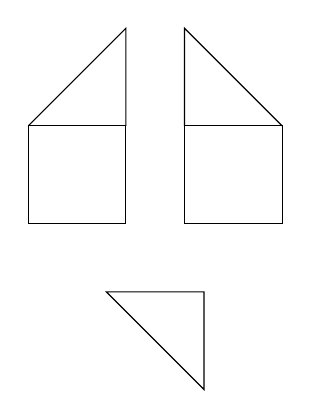
\begin{tikzpicture}[scale=0.62, font=\small]
  % 正视图（三角形直角边在右）
  \begin{scope}
    \draw (0,0) rectangle (2,2);
    \draw (0,2) -- (2,4) -- (2,2);
  \end{scope}
  % 左视图（三角形直角边在左）
  \begin{scope}[xshift=3.2cm]
    \draw (0,0) rectangle (2,2);
    \draw (0,2) -- (0,4) -- (2,2);
  \end{scope}
  % 俯视图（等腰直角三角形，直角边 2）
  \begin{scope}[yshift=-3.4cm, xshift=1.6cm]
    \draw (0,2) -- (2,2) -- (2,0) -- cycle;
  \end{scope}
\end{tikzpicture}
\end{center}
\nopagebreak[4]
\begin{gkopts}(4)
\task A．$10$
\task B．$12$
\task C．$14$
\task D．$16$
\end{gkopts}

\begin{gktip}
\textbf{注}：三视图在现行新课标中已删除。
\end{gktip}

\Needspace{4\baselineskip}
\textbf{解析}

\Needspace{5\baselineskip}
\textbf{第一步：从俯视图定底面。} 俯视图是等腰直角三角形，说明这个多面体的底面（水平投影）是一个直角边为 $2$ 的等腰直角三角形。建立坐标系（$x$ 向右、$y$ 向后、$z$ 向上），设底面三个顶点为

\nopagebreak[4]
\[A(0,2,0),\qquad B(2,2,0),\qquad C(2,0,0)\]

（直角在 $B$，与俯视图中直角在右上角对应。）

\textbf{第二步：从正视图、左视图定各点高度。}

设三条竖棱的高度分别为 $h_A$、$h_B$、$h_C$。

\begin{itemize}
\item \textbf{正视图}（投影到 $xOz$，水平轴是 $x$）：轮廓是"$2\times2$ 正方形 + 高 $2$ 的三角形"，且三角形顶点在\textbf{右上}。这说明 $x=0$ 处高度为 $2$、$x=2$ 处高度为 $4$：
\end{itemize}
\nopagebreak[4]
\[h_A=2,\qquad \max\left(h_B,h_C\right)=4\]
\begin{itemize}
\item \textbf{左视图}（投影到 $yOz$，水平轴是 $y$，\textbf{左边对应 $y$ 大即后方}）：三角形顶点在\textbf{左上}，说明 $y=2$ 处高度为 $4$、$y=0$ 处高度为 $2$：
\end{itemize}
\nopagebreak[4]
\[\max\left(h_A,h_B\right)=4,\qquad h_C=2\]

\Needspace{5\baselineskip}
联立四式：

\nopagebreak[4]
\[h_A=2,\qquad h_B=4,\qquad h_C=2\]

\Needspace{5\baselineskip}
\textbf{第三步：写出多面体。} 它是一个\textbf{底面为等腰直角三角形、三条竖棱高度分别为 $2$、$4$、$2$ 的斜三棱柱}（顶面是一个斜平面）：

\nopagebreak[4]
\[A(0,2,0),\ B(2,2,0),\ C(2,0,0);\qquad A'(0,2,2),\ B'(2,2,4),\ C'(2,0,2)\]

\textbf{第四步：找出哪些面是梯形。} 三个侧面都由两条竖棱和上下两条边围成：

\begin{center}
\begin{tabular}{lll}
\toprule
侧面 & 两条竖棱 & 形状 \\
\midrule
$ABB'A'$ & $AA'=2$，$BB'=4$（不等） & \textbf{梯形} \\
$BCC'B'$ & $BB'=4$，$CC'=2$（不等） & \textbf{梯形} \\
$ACC'A'$ & $AA'=2$，$CC'=2$（相等） & 矩形（不是梯形） \\
\bottomrule
\end{tabular}
\end{center}

上下底面 $\triangle ABC$、$\triangle A'B'C'$ 是三角形。所以\textbf{恰有两个梯形面}。

\Needspace{5\baselineskip}
\textbf{第五步：算面积。} 两条竖棱都垂直于底边，故梯形的"高"就是底边长：

\nopagebreak[4]
\[S_{ABB'A'}=\frac{AA'+BB'}2\times AB=\frac{2+4}2\times2=6\]

\nopagebreak[4]
\[S_{BCC'B'}=\frac{BB'+CC'}2\times BC=\frac{4+2}2\times2=6\]

\nopagebreak[4]
\[S_{\text{\text{梯形之和}}}=6+6=12\]

\begin{gktip}
\textbf{方法提示}：三视图还原的核心是"\textbf{俯视图定底面形状，正视图与左视图定各点高度}"。本题的巧妙之处在于两个视图各给出一半的高度信息，联立后三条竖棱的高度就唯一确定了。

学生最常见的误解是把"正方形 + 三角形"读成"棱柱上面架一个棱锥"，那样得到的立体没有梯形面，与题干矛盾 —— \textbf{题干里"有若干个面是梯形"这句话本身就是验证还原是否正确的钥匙}。

\textbf{注}：三视图在现行新课标中已删除，本题仅作历史资料。
\end{gktip}

\par\medskip

\Needspace{0.4\textheight}

\gkanswer{答案：B（$12$）}

\end{answer}
\begin{answer}
\gksolhead{8}{程序框图}

\textbf{题目}：

如图程序框图是为了求出满足 $3^{n}-2^{n}>1000$ 的最小偶数 $n$，那么在 $\Diamond$ 和 $\square$ 两个空白框中，可以分别填入\mbox{（　　）}
\nopagebreak[4]
\begin{center}% 2017 全国Ⅰ卷 理8/文10：求满足 3^n-2^n>1000 的最小偶数 n 的程序框图
% 两个空白框（菱形与左侧矩形）是题目要求填入的位置，故留白
\begin{tikzpicture}[font=\small, >=Stealth, node distance=8mm,
  box/.style={draw, minimum height=1.9em, inner xsep=7pt},
  term/.style={draw, rounded corners=7pt, minimum height=1.9em, inner xsep=9pt},
  io/.style={draw, trapezium, trapezium left angle=70, trapezium right angle=110,
             minimum height=1.9em, inner xsep=2pt},
  dec/.style={draw, diamond, aspect=2.4, inner sep=1.5pt}]
  \node[term] (start) {开始};
  \node[io, below=of start] (in) {输入 $n=0$};
  \coordinate[below=5mm of in] (merge);
  \node[box, below=2mm of merge] (calc) {$A=3^{n}-2^{n}$};
  \node[dec, below=of calc] (cond) {\phantom{$A\le1000$}};
  \node[box, left=12mm of calc, minimum width=5.2em] (blank) {\phantom{$n=n+2$}};
  \node[io, below=of cond] (out) {输出 $n$};
  \node[term, below=of out] (end) {结束};
  \draw[->] (start) -- (in);
  \draw[->] (in) -- (calc);
  \draw[->] (calc) -- (cond);
  \draw[->] (cond) -- node[right]{否} (out);
  \draw[->] (out) -- (end);
  \draw[->] (cond) -| node[below, pos=0.18]{是} (blank);
  \draw[->] (blank) |- (merge);
\end{tikzpicture}
\end{center}
\nopagebreak[4]
\begin{gkopts}(2)
\task A．$A>1000$ 和 $n=n+1$
\task B．$A>1000$ 和 $n=n+2$
\task C．$A\le1000$ 和 $n=n+1$
\task D．$A\le1000$ 和 $n=n+2$
\end{gkopts}

\begin{gktip}
\textbf{注}：程序框图（算法初步）在现行新课标中已删除。
\end{gktip}

\Needspace{4\baselineskip}
\textbf{解析}

\Needspace{5\baselineskip}
\textbf{第一步：读清流程走向。} 从图中可以看到：

\nopagebreak[4]
\[\text{\text{开始}}\to\text{\text{输入} }n=0\to\boxed{\ ?\ }\to A=3^{n}-2^{n}\to\Diamond\ ?\ \begin{cases}\text{\text{是}}\to\text{\text{回到}}\boxed{\ ?\ }\ (\text{\text{继续循环}})\\[1mm]\text{\text{否}}\to\text{\text{输出} }n\to\text{\text{结束}}\end{cases}\]

\Needspace{5\baselineskip}
\textbf{关键}：菱形的"\textbf{是}"分支是\textbf{回去继续循环}，"否"分支才输出。所以菱形里填的是"\textbf{还没达标、需要继续算}"的条件，即

\nopagebreak[4]
\[A\le1000\]

（若填 $A>1000$，则一旦达标反而会继续循环，永远不会输出，逻辑相反。）

\Needspace{5\baselineskip}
\textbf{第二步：定步长。} 题目要求的是最小\textbf{偶数} $n$，初值 $n=0$ 已是偶数，每次应加 $2$ 保持偶数：

\nopagebreak[4]
\[n=n+2\]

\textbf{验证}：$n=0\to n=2$，$A=3^{2}-2^{2}=5\le1000$，继续；$n=4$，$A=81-16=65$，继续；$n=6$，$A=729-64=665$，继续；$n=8$，$A=6561-256=6305>1000$，输出 $n=8$ 

\begin{gktip}
\textbf{方法提示}：程序框图题的判断诀窍是\textbf{看"是"分支的去向} —— 指回循环体就填"继续的条件"，指向输出就填"终止的条件"。本题四个选项两两配对，只要认准这一点就能立刻二选一。

\textbf{注}：程序框图（算法初步）在现行新课标中已删除。
\end{gktip}

\gkanswer{答案：D（$A\le1000$ 和 $n=n+2$）}

\par\medskip

\end{answer}
\begin{answer}
\gksolhead{9}{三角函数图象变换}

\textbf{题目}：

已知曲线 $C_1:y=\cos x$，$C_2:y=\sin\left(2x+\dfrac{2\pi}3\right)$，则下面结论正确的是\mbox{（　　）}

\begin{gkopts}(1)
\task A．把 $C_1$ 上各点的横坐标伸长到原来的 $2$ 倍，纵坐标不变，再把得到的曲线向右平移 $\dfrac\pi6$ 个单位长度，得到曲线 $C_2$
\task B．把 $C_1$ 上各点的横坐标伸长到原来的 $2$ 倍，纵坐标不变，再把得到的曲线向左平移 $\dfrac\pi{12}$ 个单位长度，得到曲线 $C_2$
\task C．把 $C_1$ 上各点的横坐标缩短到原来的 $\dfrac12$ 倍，纵坐标不变，再把得到的曲线向右平移 $\dfrac\pi6$ 个单位长度，得到曲线 $C_2$
\task D．把 $C_1$ 上各点的横坐标缩短到原来的 $\dfrac12$ 倍，纵坐标不变，再把得到的曲线向左平移 $\dfrac\pi{12}$ 个单位长度，得到曲线 $C_2$
\end{gkopts}

\Needspace{4\baselineskip}
\textbf{解析}

\Needspace{5\baselineskip}
\textbf{第一步：统一函数名。} 变换前后必须是同一个三角函数才好比较：

\nopagebreak[4]
\[\cos x=\sin\left(x+\frac\pi2\right)\]

\textbf{第二步：定伸缩。} 目标 $C_2$ 中 $\omega=2$，而 $C_1$ 中 $\omega=1$。$\omega$ \textbf{变大} $\Rightarrow$ 周期变小 $\Rightarrow$ 横坐标\textbf{缩短}到原来的 $\dfrac12$。故排除 A、B。

\Needspace{5\baselineskip}
缩短后得到

\nopagebreak[4]
\[y=\sin\left(2x+\frac\pi2\right)\]

\Needspace{5\baselineskip}
\textbf{第三步：定平移。} 设向左平移 $\varphi$ 个单位（$\varphi>0$ 为左移），把 $x$ 换成 $x+\varphi$：

\nopagebreak[4]
\[y=\sin\left(2(x+\varphi)+\frac\pi2\right)=\sin\left(2x+2\varphi+\frac\pi2\right)\]

\Needspace{5\baselineskip}
与目标比较：

\nopagebreak[4]
\[2\varphi+\frac\pi2=\frac{2\pi}3\ \Longrightarrow\ 2\varphi=\frac{2\pi}3-\frac\pi2=\frac{4\pi-3\pi}6=\frac\pi6\ \Longrightarrow\ \varphi=\frac\pi{12}\]

$\varphi>0$，故是向\textbf{左}平移 $\dfrac\pi{12}$ 个单位。

\begin{gktip}
\textbf{方法提示}：三角变换题的两大坑：

1. \textbf{"横坐标伸长到 $2$ 倍"对应 $\omega$ 减半，"缩短到 $\dfrac12$"对应 $\omega$ 加倍} —— 与直觉相反，因为 $\omega$ 在括号里。
2. \textbf{先伸缩后平移时，平移量要除以 $\omega$}。本题中相位差是 $\dfrac{2\pi}3-\dfrac\pi2=\dfrac\pi6$，但平移量是 $\dfrac\pi6\div2=\dfrac\pi{12}$。选项 C 的 $\dfrac\pi6$ 正是为忘记除以 $\omega$ 的人准备的。
\end{gktip}

\gkanswer{答案：D}

\par\medskip

\end{answer}
\begin{answer}
\gksolhead{10}{抛物线两条垂直焦点弦}

\textbf{题目}：

已知 $F$ 为抛物线 $C:y^{2}=4x$ 的焦点，过 $F$ 作两条互相垂直的直线 $l_1$，$l_2$，直线 $l_1$ 与 $C$ 交于 $A$，$B$ 两点，直线 $l_2$ 与 $C$ 交于 $D$，$E$ 两点，则 $|AB|+|DE|$ 的最小值为\mbox{（　　）}

\begin{gkopts}(4)
\task A．$16$
\task B．$14$
\task C．$12$
\task D．$10$
\end{gkopts}

\Needspace{4\baselineskip}
\textbf{解析}

\Needspace{5\baselineskip}
\textbf{第一步：焦点弦长公式。} 对抛物线 $y^{2}=2px$，过焦点且倾斜角为 $\theta$ 的弦长为

\nopagebreak[4]
\[L=\frac{2p}{\sin^{2}\theta}\]

\Needspace{5\baselineskip}
本题 $2p=4$，故

\nopagebreak[4]
\[|AB|=\frac4{\sin^{2}\theta}\]

\Needspace{5\baselineskip}
\textbf{第二步：写出另一条。} $l_2\perp l_1$，倾斜角为 $\theta+\dfrac\pi2$，而 $\sin\left(\theta+\dfrac\pi2\right)=\cos\theta$：

\nopagebreak[4]
\[|DE|=\frac4{\cos^{2}\theta}\]

（注意两条弦都必须与抛物线交于两点，故 $\theta\ne0,\dfrac\pi2$，$\sin\theta\cos\theta\ne0$。）

\Needspace{5\baselineskip}
\textbf{第三步：求和的最小值。}

\nopagebreak[4]
\[|AB|+|DE|=\frac4{\sin^{2}\theta}+\frac4{\cos^{2}\theta}=\frac{4\left(\cos^{2}\theta+\sin^{2}\theta\right)}{\sin^{2}\theta\cos^{2}\theta}=\frac4{\sin^{2}\theta\cos^{2}\theta}\]

\Needspace{5\baselineskip}
用二倍角 $\sin\theta\cos\theta=\dfrac12\sin2\theta$：

\nopagebreak[4]
\[=\frac4{\frac14\sin^{2}2\theta}=\frac{16}{\sin^{2}2\theta}\ \ge\ 16\]

等号当 $\sin^{2}2\theta=1$，即 $\theta=\dfrac\pi4$ 时取到（此时两条弦关于 $x$ 轴对称，长度都是 $8$）。

\begin{gktip}
\textbf{方法提示}：\textbf{焦点弦长公式 $L=\dfrac{2p}{\sin^{2}\theta}$ 必须记住}，它把这类题从"设直线—联立—韦达—弦长公式"的四步计算压缩成一步。

若不记得公式，也可设 $l_1:x=my+1$，联立得 $y^{2}-4my-4=0$，$|AB|=\sqrt{1+m^{2}}\cdot\left|y_1-y_2\right|=4\left(1+m^{2}\right)$；$l_2$ 对应把 $m$ 换成 $-\dfrac1m$，得 $|DE|=4\left(1+\dfrac1{m^{2}}\right)$。和为 $8+4\left(m^{2}+\dfrac1{m^{2}}\right)\ge8+8=16$。
\end{gktip}

\gkanswer{答案：A（$16$）}

\par\medskip

\end{answer}
\begin{answer}
\gksolhead{11}{指对数比大小}

\textbf{题目}：

设 $x$，$y$，$z$ 为正数，且 $2^{x}=3^{y}=5^{z}$，则\mbox{（　　）}

\begin{gkopts}(4)
\task A．$2x<3y<5z$
\task B．$5z<2x<3y$
\task C．$3y<5z<2x$
\task D．$3y<2x<5z$
\end{gkopts}

\Needspace{4\baselineskip}
\textbf{解析}

\Needspace{5\baselineskip}
\textbf{第一步：设公共值取对数。} 令 $2^{x}=3^{y}=5^{z}=k$。因 $x,y,z>0$，必有 $k>1$，故 $\ln k>0$。取自然对数：

\nopagebreak[4]
\[x=\frac{\ln k}{\ln2},\qquad y=\frac{\ln k}{\ln3},\qquad z=\frac{\ln k}{\ln5}\]

\Needspace{5\baselineskip}
于是

\nopagebreak[4]
\[2x=\frac{2\ln k}{\ln2},\qquad 3y=\frac{3\ln k}{\ln3},\qquad 5z=\frac{5\ln k}{\ln5}\]

\Needspace{5\baselineskip}
因 $\ln k>0$ 是公因子，只需比较

\nopagebreak[4]
\[\frac2{\ln2},\qquad \frac3{\ln3},\qquad \frac5{\ln5}\]

\textbf{第二步：两两比较（交叉相乘化为对数比较）。}

\Needspace{5\baselineskip}
\textbf{比 $2x$ 与 $3y$}：

\nopagebreak[4]
\[\frac2{\ln2}\ \text{vs}\ \frac3{\ln3}\iff 2\ln3\ \text{vs}\ 3\ln2\iff \ln9\ \text{vs}\ \ln8\]

\Needspace{5\baselineskip}
$9>8\Rightarrow\ln9>\ln8\Rightarrow\dfrac2{\ln2}>\dfrac3{\ln3}$，即

\nopagebreak[4]
\[2x>3y\]

\Needspace{5\baselineskip}
\textbf{比 $2x$ 与 $5z$}：

\nopagebreak[4]
\[\frac2{\ln2}\ \text{vs}\ \frac5{\ln5}\iff 2\ln5\ \text{vs}\ 5\ln2\iff \ln25\ \text{vs}\ \ln32\]

\Needspace{5\baselineskip}
$25<32\Rightarrow\ln25<\ln32\Rightarrow\dfrac2{\ln2}<\dfrac5{\ln5}$，即

\nopagebreak[4]
\[2x<5z\]

\Needspace{5\baselineskip}
合并：

\nopagebreak[4]
\[3y<2x<5z\]

\begin{gktip}
\textbf{方法提示}：$a\ln b$ 与 $b\ln a$ 的比较，一律化成 $\ln b^{a}$ 与 $\ln a^{b}$，也就是比较 $b^{a}$ 与 $a^{b}$ 这两个整数的大小 —— $9$ vs $8$、$25$ vs $32$ 一眼就能判断，比估算 $\ln2\approx0.693$ 之类可靠得多。
\end{gktip}

\gkanswer{答案：D（$3y<2x<5z$）}

\par\medskip

\end{answer}
\begin{answer}
\gksolhead{12}{分组数列 · 软件激活码}

\textbf{题目}：

几位大学生响应国家的创业号召，开发了一款应用软件。为激发大家学习数学的兴趣，他们推出了"解数学题获取软件激活码"的活动。这款软件的激活码为下面数学问题的答案：已知数列 $1$，$1$，$2$，$1$，$2$，$4$，$1$，$2$，$4$，$8$，$1$，$2$，$4$，$8$，$16$，$\cdots$，其中第一项是 $2^{0}$，接下来的两项是 $2^{0}$，$2^{1}$，再接下来的三项是 $2^{0}$，$2^{1}$，$2^{2}$，依此类推。求满足如下条件的最小整数 $N$：$N>100$ 且该数列的前 $N$ 项和为 $2$ 的整数幂。那么该款软件的激活码是\mbox{（　　）}

\begin{gkopts}(4)
\task A．$440$
\task B．$330$
\task C．$220$
\task D．$110$
\end{gkopts}

\Needspace{4\baselineskip}
\textbf{解析}

\Needspace{5\baselineskip}
\textbf{第一步：算每组的和。} 第 $k$ 组共 $k$ 项，是公比 $2$ 的等比数列：

\nopagebreak[4]
\[T_k=2^{0}+2^{1}+\cdots+2^{k-1}=2^{k}-1\]

\Needspace{5\baselineskip}
\textbf{第二步：算前 $k$ 组的总和。}

\nopagebreak[4]
\[\sum_{j=1}^{k}T_j=\sum_{j=1}^{k}\left(2^{j}-1\right)=\left(2^{k+1}-2\right)-k\]

前 $k$ 组共 $\dfrac{k(k+1)}2$ 项。

\Needspace{5\baselineskip}
\textbf{第三步：写出一般的 $S_N$。} 设 $N$ 项 $=$ 前 $k$ 组 $+$ 第 $(k+1)$ 组的前 $m$ 项（$0\le m\le k+1$），即

\nopagebreak[4]
\[N=\frac{k(k+1)}2+m\]

\nopagebreak[4]
\[S_N=\left(2^{k+1}-2-k\right)+\left(2^{m}-1\right)=2^{k+1}+2^{m}-(k+3)\]

\textbf{第四步：什么时候 $S_N$ 是 $2$ 的幂？}

\Needspace{5\baselineskip}
设 $S_N=2^{t}$，即

\nopagebreak[4]
\[2^{k+1}+2^{m}-(k+3)=2^{t}\]

\textbf{注意到一个显然的解：若 $k+3=2^{m}$，则 $S_N=2^{k+1}$，正是 $2$ 的幂。}

下面说明\textbf{只有这种情况}：

\begin{itemize}
\item 若 $t\ge k+2$：则 $2^{t}-2^{k+1}\ge2^{k+1}$，需 $2^{m}-(k+3)\ge2^{k+1}$。但 $m\le k+1$ 给出 $2^{m}\le2^{k+1}$，故 $2^{m}-(k+3)<2^{k+1}$，矛盾。
\item 若 $t\le k$：则 $2^{t}\le2^{k}$。而 $S_N\ge2^{k+1}+2^{0}-(k+3)=2^{k+1}-k-2$，对 $k\ge2$ 有 $2^{k+1}-k-2>2^{k}$，矛盾。
\item 故只能 $t=k+1$，此时 $2^{m}=k+3$。
\end{itemize}

\textbf{第五步：枚举。} 由 $k=2^{m}-3$ 得

\begin{center}
\begin{tabular}{ccc}
\toprule
$m$ & $k=2^{m}-3$ & $N=\dfrac{k(k+1)}2+m$ \\
\midrule
$2$ & $1$ & $1+2=3$ \\
$3$ & $5$ & $15+3=18$ \\
$4$ & $13$ & $91+4=95$ \\
$5$ & $29$ & $435+5=440$ \\
\bottomrule
\end{tabular}
\end{center}

（$m=1$ 给出 $k=-1$，无意义。还需 $m\le k+1$：$m=5,k=29$ 显然满足。）

\Needspace{5\baselineskip}
要求 $N>100$，最小的是

\nopagebreak[4]
\[N=440\]

\textbf{验证}（$k=29$，$m=5$）：$S_N=2^{30}+2^{5}-32=2^{30}$  确实是 $2$ 的幂。

\begin{gktip}
\textbf{方法提示}：本题是当年全国卷的"压轴选择题"，难点有两处：

1. \textbf{正确写出 $S_N$ 的一般表达式}（要把"前 $k$ 组完整 + 第 $k+1$ 组的前 $m$ 项"这个结构说清楚）；
2. \textbf{论证 $k+3=2^{m}$ 是唯一可能}（不能只凭"凑出来一个就是答案"）。

考场上时间紧张时，可以先猜"$k+3$ 是 $2$ 的幂"这条主线快速枚举出 $3,18,95,440$，选出第一个大于 $100$ 的即可 —— 四个选项中只有 $440$ 出现在这个序列里，也是一种验证。
\end{gktip}

\gkanswer{答案：A（$440$）}

\par\medskip

\end{answer}
\gkpart{二、填空题}

\begin{answer}
\gksolhead{13}{向量的模}

\textbf{题目}：

已知向量 $\boldsymbol a$，$\boldsymbol b$ 的夹角为 $60^\circ$，$|\boldsymbol a|=2$，$|\boldsymbol b|=1$，则 $|\boldsymbol a+2\boldsymbol b|=$ \gkblank{}．

\Needspace{4\baselineskip}
\textbf{解析}

\Needspace{5\baselineskip}
先算数量积：

\nopagebreak[4]
\[\boldsymbol a\cdot\boldsymbol b=|\boldsymbol a||\boldsymbol b|\cos60^\circ=2\times1\times\frac12=1\]

\Needspace{5\baselineskip}
再对模平方展开：

\nopagebreak[4]
\[|\boldsymbol a+2\boldsymbol b|^{2}=|\boldsymbol a|^{2}+4\,\boldsymbol a\cdot\boldsymbol b+4|\boldsymbol b|^{2}=4+4\times1+4\times1=12\]

\nopagebreak[4]
\[|\boldsymbol a+2\boldsymbol b|=\sqrt{12}=2\sqrt3\]

\begin{gktip}
\textbf{方法提示}：求向量的模一律先平方，用 $|\boldsymbol u|^{2}=\boldsymbol u\cdot\boldsymbol u$ 展开，最后再开方。
\end{gktip}

\gkanswer{答案：$2\sqrt3$}

\par\medskip

\end{answer}
\begin{answer}
\gksolhead{14}{线性规划}

\textbf{题目}：

设 $x$，$y$ 满足约束条件 $\begin{cases}x+2y\le1\\ 2x+y\ge-1\\ x-y\le0\end{cases}$，则 $z=3x-2y$ 的最小值为 \gkblank{}．

\Needspace{4\baselineskip}
\textbf{解析}

\textbf{求可行域顶点}（三条边界直线两两联立）：

\begin{itemize}
\item $x+2y=1$ 与 $x-y=0$：代入 $x=y$ 得 $3y=1$，顶点 $\left(\dfrac13,\dfrac13\right)$；
\item $2x+y=-1$ 与 $x-y=0$：代入 $x=y$ 得 $3y=-1$，顶点 $\left(-\dfrac13,-\dfrac13\right)$；
\item $x+2y=1$ 与 $2x+y=-1$：解得 $x=-1$，$y=1$，顶点 $(-1,1)$。
\end{itemize}

（三点都满足全部约束，可行域是这个三角形。）

\Needspace{0.25\textheight}

\textbf{代入目标函数}：

\begin{center}
\begin{tabular}{cc}
\toprule
顶点 & $z=3x-2y$ \\
\midrule
$\left(\dfrac13,\dfrac13\right)$ & $1-\dfrac23=\dfrac13$ \\
$\left(-\dfrac13,-\dfrac13\right)$ & $-1+\dfrac23=-\dfrac13$ \\
$(-1,1)$ & $-3-2=\boxed{-5}$ \\
\bottomrule
\end{tabular}
\end{center}

\gkanswer{答案：$-5$}

\par\medskip

\end{answer}
\begin{answer}
\gksolhead{15}{双曲线离心率}

\textbf{题目}：

已知双曲线 $C:\dfrac{x^{2}}{a^{2}}-\dfrac{y^{2}}{b^{2}}=1\ (a>0,\ b>0)$ 的右顶点为 $A$，以 $A$ 为圆心、$b$ 为半径作圆 $A$，圆 $A$ 与双曲线 $C$ 的一条渐近线交于 $M$，$N$ 两点。若 $\angle MAN=60^\circ$，则 $C$ 的离心率为 \gkblank{}．

\Needspace{4\baselineskip}
\textbf{解析}

\textbf{第一步：由 $\angle MAN=60^\circ$ 算圆心到弦的距离。}

\Needspace{5\baselineskip}
$AM=AN=b$（都是半径），夹角 $60^\circ$，故 $\triangle AMN$ 是\textbf{等边三角形}。等边三角形中，顶点到对边的距离（即高）为

\nopagebreak[4]
\[d=b\cdot\cos30^\circ=\frac{\sqrt3}2b\]

这个 $d$ 就是圆心 $A$ 到渐近线的距离。

\textbf{第二步：直接算 $A$ 到渐近线的距离。}

\Needspace{5\baselineskip}
右顶点 $A(a,0)$，渐近线取 $y=\dfrac bax$，即 $bx-ay=0$：

\nopagebreak[4]
\[d=\frac{|ba-a\cdot0|}{\sqrt{b^{2}+a^{2}}}=\frac{ab}{c}\]

（用了 $a^{2}+b^{2}=c^{2}$。）

\Needspace{5\baselineskip}
\textbf{第三步：联立。}

\nopagebreak[4]
\[\frac{ab}c=\frac{\sqrt3}2b\ \Longrightarrow\ \frac ac=\frac{\sqrt3}2\ \Longrightarrow\ e=\frac ca=\frac2{\sqrt3}=\frac{2\sqrt3}3\]

\begin{gktip}
\textbf{方法提示}：$b$ 在两边约掉了，这是本题的设计巧思 —— \textbf{半径恰好取成 $b$，使得离心率与 $b$ 无关}。另外"顶点到渐近线的距离 $=\dfrac{ab}c$"和"焦点到渐近线的距离 $=b$"是一对常用结论，值得一起记。
\end{gktip}

\gkanswer{答案：$\dfrac{2\sqrt3}3$}

\par\medskip

\end{answer}
\begin{answer}
\gksolhead{16}{折纸最值}

\textbf{题目}：

如图，圆形纸片的圆心为 $O$，半径为 $5\ \mathrm{cm}$，该纸片上的等边三角形 $ABC$ 的中心为 $O$。$D$，$E$，$F$ 为圆 $O$ 上的点，$\triangle DBC$，$\triangle ECA$，$\triangle FAB$ 分别是以 $BC$，$CA$，$AB$ 为底边的等腰三角形。沿虚线剪开后，分别以 $BC$，$CA$，$AB$ 为折痕折起 $\triangle DBC$，$\triangle ECA$，$\triangle FAB$，使得 $D$，$E$，$F$ 重合，得到三棱锥。当 $\triangle ABC$ 的边长变化时，所得三棱锥体积（单位：$\mathrm{cm}^{3}$）的最大值为 \gkblank{}．
\nopagebreak[4]
\begin{center}% 2017 全国Ⅰ卷 理16：圆形纸片（半径 5）与内接等边三角形 ABC，
% D、E、F 为圆上的点，分别与 BC、CA、AB 构成待折起的等腰三角形
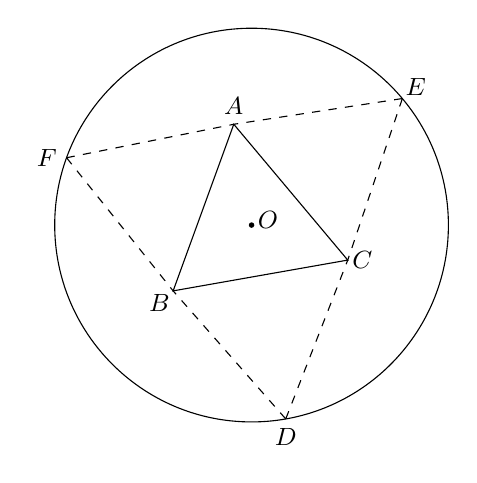
\begin{tikzpicture}[scale=1.0, font=\small]
  \def\R{2.5}      % 圆半径（示意比例）
  \def\r{1.3}      % 三角形中心到顶点距离
  \draw (0,0) circle (\R);
  \coordinate (A) at (100:\r);
  \coordinate (B) at (220:\r);
  \coordinate (C) at (-20:\r);
  \coordinate (D) at (280:\R);
  \coordinate (E) at (40:\R);
  \coordinate (F) at (160:\R);
  \draw (A) -- (B) -- (C) -- cycle;
  \draw[dashed] (D) -- (B) (D) -- (C);
  \draw[dashed] (E) -- (C) (E) -- (A);
  \draw[dashed] (F) -- (A) (F) -- (B);
  \fill (0,0) circle (1pt);
  \node[right, inner sep=1.5pt] at (0.02,0.06) {$O$};
  \node[above] at (A) {$A$};
  \node[below left, inner sep=1pt] at (B) {$B$};
  \node[right, inner sep=1.5pt] at (C) {$C$};
  \node[below] at (D) {$D$};
  \node[above right, inner sep=1pt] at (E) {$E$};
  \node[left] at (F) {$F$};
\end{tikzpicture}
\end{center}
\nopagebreak[4]
\Needspace{4\baselineskip}
\textbf{解析}

\textbf{第一步：设合适的变量。} 设 $\triangle ABC$ 的中心 $O$ 到各边的距离（即内切圆半径）为 $t$，则由等边三角形的性质：

\begin{itemize}
\item 边长 $a=2\sqrt3\,t$（因为内切圆半径 $t=\dfrac a{2\sqrt3}$）；
\item 中心到顶点的距离 $OA=2t$；
\item 面积 $S_{\triangle ABC}=\dfrac{\sqrt3}4a^{2}=\dfrac{\sqrt3}4\times12t^{2}=3\sqrt3\,t^{2}$。
\end{itemize}

\Needspace{5\baselineskip}
\textbf{第二步：算斜高。} 设 $BC$ 的中点为 $M$，则 $OM=t$，且 $D$、$O$、$M$ 三点共线（$\triangle DBC$ 是等腰三角形，$D$ 在 $BC$ 的中垂线上，而该中垂线过 $O$）。$D$ 在圆上、位于 $BC$ 的\textbf{外侧}，故

\nopagebreak[4]
\[MD=OD-OM=5-t\]

折起后 $MD$ 成为三棱锥的\textbf{斜高}（顶点到底面边 $BC$ 中点的距离），它在折叠中长度不变。

\Needspace{5\baselineskip}
\textbf{第三步：算锥高。} 折起后顶点落在 $O$ 的正上方（由对称性），锥高 $h$ 满足

\nopagebreak[4]
\[h^{2}=MD^{2}-OM^{2}=(5-t)^{2}-t^{2}=25-10t\]

\nopagebreak[4]
\[h=\sqrt{25-10t}\]

（需 $0<t<\dfrac52$。）

\Needspace{5\baselineskip}
\textbf{第四步：写出体积并求最值。}

\nopagebreak[4]
\[V=\frac13S_{\triangle ABC}\cdot h=\frac13\times3\sqrt3\,t^{2}\times\sqrt{25-10t}=\sqrt3\,t^{2}\sqrt{25-10t}\]

\Needspace{5\baselineskip}
平方后求最值（避免根号）：

\nopagebreak[4]
\[V^{2}=3t^{4}(25-10t)=75t^{4}-30t^{5}\]

\nopagebreak[4]
\[\left(V^{2}\right)'=300t^{3}-150t^{4}=150t^{3}(2-t)\]

\Needspace{5\baselineskip}
在 $\left(0,\dfrac52\right)$ 上，$t<2$ 时导数为正、$t>2$ 时为负，故 $t=2$ 是最大值点：

\nopagebreak[4]
\[V^{2}\Big|_{t=2}=75\times16-30\times32=1200-960=240\]

\nopagebreak[4]
\[V_{\max}=\sqrt{240}=4\sqrt{15}\]

\textbf{验算}（$t=2$）：边长 $a=4\sqrt3$，$OA=4<5$（顶点确实在圆内 ），$MD=3$，$h=\sqrt{9-4}=\sqrt5$，$S=\dfrac{\sqrt3}4\times48=12\sqrt3$，$V=\dfrac13\times12\sqrt3\times\sqrt5=4\sqrt{15}$ 

\begin{gktip}
\textbf{方法提示}：这是折叠类最值题的典范，三个关键点：

1. \textbf{选对变量}。用"中心到边的距离 $t$"比用边长 $a$ 简洁得多，因为 $MD=5-t$ 直接就是 $t$ 的一次式。
2. \textbf{认清哪个量在折叠中不变} —— 是斜高 $MD$，不是锥高。$h=\sqrt{MD^{2}-OM^{2}}$ 里 $t^{2}$ 恰好抵消，得到干净的 $\sqrt{25-10t}$，这是本题能算下去的关键。
3. \textbf{对 $V^{2}$ 求导而不是对 $V$ 求导}，可以避开根号的求导。
\end{gktip}

\gkanswer{答案：$4\sqrt{15}$}

\par\medskip

\end{answer}
\gkpart{三、解答题}

\begin{answer}
\gksolhead{17}{12 分，解三角形}

\textbf{题目}（12 分）：

$\triangle ABC$ 的内角 $A$，$B$，$C$ 的对边分别为 $a$，$b$，$c$，已知 $\triangle ABC$ 的面积为 $\dfrac{a^{2}}{3\sin A}$。

  (1) 求 $\sin B\sin C$；

  (2) 若 $6\cos B\cos C=1$，$a=3$，求 $\triangle ABC$ 的周长。

\Needspace{4\baselineskip}
\textbf{解析}

\gksubpart{(1) 求 $\sin B\sin C$}

\Needspace{5\baselineskip}
面积公式给出

\nopagebreak[4]
\[\frac12bc\sin A=\frac{a^{2}}{3\sin A}\]

\Needspace{5\baselineskip}
两边乘 $\sin A$：

\nopagebreak[4]
\[\frac12bc\sin^{2}A=\frac{a^{2}}3\ \Longrightarrow\ bc\sin^{2}A=\frac{2a^{2}}3\]

\Needspace{5\baselineskip}
\textbf{用正弦定理把边全部换成角}（设外接圆半径 $R$）：$a=2R\sin A$，$b=2R\sin B$，$c=2R\sin C$：

\nopagebreak[4]
\[4R^{2}\sin B\sin C\cdot\sin^{2}A=\frac23\cdot4R^{2}\sin^{2}A\]

\Needspace{5\baselineskip}
约去 $4R^{2}\sin^{2}A$（非零）：

\nopagebreak[4]
\[\sin B\sin C=\frac23\]

\gksubpart{(2) 求周长}

\Needspace{5\baselineskip}
\textbf{第一步：定角 $A$。} 由已知 $\cos B\cos C=\dfrac16$，结合 (1)：

\nopagebreak[4]
\[\cos(B+C)=\cos B\cos C-\sin B\sin C=\frac16-\frac23=-\frac12\]

\Needspace{5\baselineskip}
$B+C\in(0,\pi)$，故 $B+C=\dfrac{2\pi}3$，从而

\nopagebreak[4]
\[A=\pi-\frac{2\pi}3=\frac\pi3,\qquad \sin A=\frac{\sqrt3}2\]

\Needspace{5\baselineskip}
\textbf{第二步：求 $bc$。} 由 $a=3$ 与正弦定理：

\nopagebreak[4]
\[2R=\frac a{\sin A}=\frac3{\frac{\sqrt3}2}=2\sqrt3\ \Longrightarrow\ 4R^{2}=12\]

\Needspace{5\baselineskip}
由 (1)：

\nopagebreak[4]
\[bc=4R^{2}\sin B\sin C=12\times\frac23=8\]

\Needspace{5\baselineskip}
\textbf{第三步：求 $b+c$。} 余弦定理：

\nopagebreak[4]
\[a^{2}=b^{2}+c^{2}-2bc\cos A\ \Longrightarrow\ 9=b^{2}+c^{2}-2\times8\times\frac12=b^{2}+c^{2}-8\]

\nopagebreak[4]
\[b^{2}+c^{2}=17\]

\nopagebreak[4]
\[(b+c)^{2}=b^{2}+c^{2}+2bc=17+16=33\ \Longrightarrow\ b+c=\sqrt{33}\]

\Needspace{5\baselineskip}
\textbf{周长}：

\nopagebreak[4]
\[a+b+c=3+\sqrt{33}\]

\begin{gktip}
\textbf{方法提示}：第 (2) 问的突破口是"\textbf{$\sin B\sin C$ 与 $\cos B\cos C$ 都给了，立刻想到两角和的余弦公式}"。这个组合几乎是在明示 $\cos(B+C)$。

最后一步只需 $b+c$ 而不需要分别求出 $b$、$c$ —— 用 $(b+c)^{2}=b^{2}+c^{2}+2bc$ 一步到位，比解方程组快得多。
\end{gktip}

\gkanswer{答案（1）：$\sin B\sin C=\dfrac23$}

\gkanswer{答案（2）：周长 $=3+\sqrt{33}$}

\par\medskip

\end{answer}
\begin{answer}
\gksolhead{18}{12 分，立体几何}

\textbf{题目}（12 分）：

如图，在四棱锥 $P\text{-}ABCD$ 中，$AB\parallel CD$，且 $\angle BAP=\angle CDP=90^\circ$。
\nopagebreak[4]
\begin{center}% 2017 全国Ⅰ卷 理18/文18：四棱锥 P-ABCD（AB∥CD，∠BAP=∠CDP=90°）
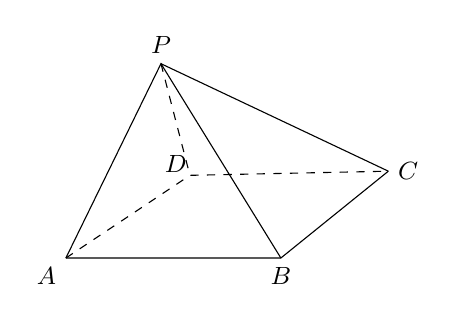
\begin{tikzpicture}[scale=1.05, font=\small]
  \coordinate (P) at (1.15,2.35);
  \coordinate (A) at (0,0);
  \coordinate (B) at (2.6,0);
  \coordinate (C) at (3.9,1.05);
  \coordinate (D) at (1.5,1.0);
  \draw (A) -- (B) -- (C);
  \draw (A) -- (P) -- (B);
  \draw (P) -- (C);
  \draw[dashed] (A) -- (D) -- (C);
  \draw[dashed] (P) -- (D);
  \node[above] at (P) {$P$};
  \node[below left] at (A) {$A$};
  \node[below] at (B) {$B$};
  \node[right] at (C) {$C$};
  \node[above left, inner sep=1pt] at (D) {$D$};
\end{tikzpicture}
\end{center}
\nopagebreak[4]
  (1) 证明：平面 $PAB\perp$ 平面 $PAD$；

  (2) 若 $PA=PD=AB=DC$，$\angle APD=90^\circ$，求二面角 $A\text{-}PB\text{-}C$ 的余弦值。

\Needspace{4\baselineskip}
\textbf{解析}

\gksubpart{(1) 证明平面 $PAB\perp$ 平面 $PAD$}

\Needspace{5\baselineskip}
\textbf{第一步：由两个直角得两条垂直关系。}

\nopagebreak[4]
\[\angle BAP=90^\circ\ \Longrightarrow\ AB\perp AP\]

\nopagebreak[4]
\[\angle CDP=90^\circ\ \Longrightarrow\ CD\perp PD\]

\Needspace{5\baselineskip}
\textbf{第二步：用平行"搬运"垂直关系。} 因 $AB\parallel CD$，而 $CD\perp PD$，故

\nopagebreak[4]
\[AB\perp PD\]

\Needspace{5\baselineskip}
\textbf{第三步：判定线面垂直。} 现在 $AB$ 同时垂直于 $AP$ 和 $PD$，而

\nopagebreak[4]
\[AP\cap PD=P,\qquad AP,\ PD\subset\text{\text{平面} }PAD\]

\Needspace{5\baselineskip}
由线面垂直判定定理：

\nopagebreak[4]
\[AB\perp\text{\text{平面} }PAD\]

\Needspace{5\baselineskip}
\textbf{第四步：升级为面面垂直。} $AB\subset$ 平面 $PAB$，故

\nopagebreak[4]
\[\text{\text{平面} }PAB\perp\text{\text{平面} }PAD\qquad\blacksquare\]

\gksubpart{(2) 求二面角 $A\text{-}PB\text{-}C$ 的余弦值}

设 $PA=PD=AB=DC=2$（题目只给了相等关系，可设具体值）。

\Needspace{5\baselineskip}
由 $\angle APD=90^\circ$ 与 $PA=PD=2$：

\nopagebreak[4]
\[AD=\sqrt{PA^{2}+PD^{2}}=2\sqrt2\]

\textbf{建系}：由 (1) 知 $AB\perp$ 平面 $PAD$，故 $AB\perp AD$ 且 $AB\perp AP$，取 $AB$ 方向为一个坐标轴最方便。

以 $A$ 为原点，$AD$ 方向为 $x$ 轴，$AB$ 方向为 $y$ 轴，平面 $PAD$ 内垂直于 $AD$ 的方向为 $z$ 轴：

\begin{itemize}
\item $A(0,0,0)$，$D\left(2\sqrt2,0,0\right)$，$B(0,2,0)$；
\item $P$ 在平面 $PAD$（即 $y=0$ 平面）内，$PA=PD=2$ 说明 $P$ 在 $AD$ 的中垂线上，横坐标为 $\sqrt2$；由 $PA=2$ 得竖坐标 $\sqrt{4-2}=\sqrt2$，故
\end{itemize}
\nopagebreak[4]
\[P\left(\sqrt2,\ 0,\ \sqrt2\right)\]
\begin{itemize}
\item $C$：$CD\parallel AB$ 且 $DC=AB=2$，故 $\overrightarrow{DC}=\overrightarrow{AB}=(0,2,0)$，
\end{itemize}
\nopagebreak[4]
\[C\left(2\sqrt2,\ 2,\ 0\right)\]

\Needspace{5\baselineskip}
\textbf{求两个半平面的法向量}：

\nopagebreak[4]
\[\overrightarrow{PA}=\left(-\sqrt2,0,-\sqrt2\right),\quad \overrightarrow{PB}=\left(-\sqrt2,2,-\sqrt2\right),\quad \overrightarrow{PC}=\left(\sqrt2,2,-\sqrt2\right)\]

\Needspace{5\baselineskip}
\textbf{平面 $APB$ 的法向量} $\boldsymbol n_1=\overrightarrow{PA}\times\overrightarrow{PB}$：

\nopagebreak[4]
\[\boldsymbol n_1=\begin{vmatrix}\boldsymbol i&\boldsymbol j&\boldsymbol k\\-\sqrt2&0&-\sqrt2\\-\sqrt2&2&-\sqrt2\end{vmatrix}\]

\begin{itemize}
\item $\boldsymbol i$ 分量：$0\times(-\sqrt2)-(-\sqrt2)\times2=2\sqrt2$
\item $\boldsymbol j$ 分量：$-\left[(-\sqrt2)(-\sqrt2)-(-\sqrt2)(-\sqrt2)\right]=-[2-2]=0$
\item $\boldsymbol k$ 分量：$(-\sqrt2)\times2-0\times(-\sqrt2)=-2\sqrt2$
\end{itemize}

\nopagebreak[4]
\[\boldsymbol n_1=\left(2\sqrt2,\ 0,\ -2\sqrt2\right)\ \sim\ (1,\ 0,\ -1)\]

\Needspace{5\baselineskip}
\textbf{平面 $PBC$ 的法向量} $\boldsymbol n_2=\overrightarrow{PB}\times\overrightarrow{PC}$：

\nopagebreak[4]
\[\boldsymbol n_2=\begin{vmatrix}\boldsymbol i&\boldsymbol j&\boldsymbol k\\-\sqrt2&2&-\sqrt2\\ \sqrt2&2&-\sqrt2\end{vmatrix}\]

\begin{itemize}
\item $\boldsymbol i$ 分量：$2\times(-\sqrt2)-(-\sqrt2)\times2=-2\sqrt2+2\sqrt2=0$
\item $\boldsymbol j$ 分量：$-\left[(-\sqrt2)(-\sqrt2)-(-\sqrt2)(\sqrt2)\right]=-[2+2]=-4$
\item $\boldsymbol k$ 分量：$(-\sqrt2)\times2-2\times\sqrt2=-4\sqrt2$
\end{itemize}

\nopagebreak[4]
\[\boldsymbol n_2=\left(0,\ -4,\ -4\sqrt2\right)\ \sim\ \left(0,\ 1,\ \sqrt2\right)\]

\Needspace{5\baselineskip}
\textbf{求夹角}：

\nopagebreak[4]
\[\cos\left\langle\boldsymbol n_1,\boldsymbol n_2\right\rangle=\frac{\boldsymbol n_1\cdot\boldsymbol n_2}{\left|\boldsymbol n_1\right|\left|\boldsymbol n_2\right|}=\frac{1\times0+0\times1+(-1)\times\sqrt2}{\sqrt2\times\sqrt3}=\frac{-\sqrt2}{\sqrt6}=-\frac1{\sqrt3}=-\frac{\sqrt3}3\]

\textbf{定符号}：从图形看，$A$ 与 $C$ 分居棱 $PB$ 的两侧且张开较大，二面角 $A\text{-}PB\text{-}C$ 是\textbf{钝角}，故余弦值取负。

\begin{gktip}
\textbf{方法提示}：本题第 (2) 问的关键在于\textbf{建系前先把 $P$ 的位置算出来}。由 $PA=PD$ 知 $P$ 在 $AD$ 的中垂面上，由 $\angle APD=90^\circ$ 知 $\triangle APD$ 是等腰直角三角形 —— 两条信息合起来，$P$ 的坐标就唯一确定了。

二面角的\textbf{正负号}不能只看法向量夹角的计算结果（法向量方向可以任取），必须结合图形判断是锐角还是钝角。本题从图上看 $A$、$C$ 位于棱的两侧且几乎"背对背"，是钝角。
\end{gktip}

\gkanswer{答案（1）：见解析版}

\gkanswer{答案（2）：$-\dfrac{\sqrt3}3$}

\par\medskip

\end{answer}
\begin{answer}
\gksolhead{19}{12 分，正态分布与统计推断}

\textbf{题目}（12 分）：

为了监控某种零件的一条生产线的生产过程，检验员每天从该生产线上随机抽取 $16$ 个零件，并测量其尺寸（单位：$\mathrm{cm}$）。根据长期生产经验，可以认为这条生产线正常状态下生产的零件的尺寸服从正态分布 $N\left(\mu,\sigma^{2}\right)$。

  (1) 假设生产状态正常，记 $X$ 表示一天内抽取的 $16$ 个零件中其尺寸在 $(\mu-3\sigma,\ \mu+3\sigma)$ 之外的零件数，求 $P(X\ge1)$ 及 $X$ 的数学期望；

  (2) 一天内抽检零件中，如果出现了尺寸在 $(\mu-3\sigma,\ \mu+3\sigma)$ 之外的零件，就认为这条生产线在这一天的生产过程可能出现了异常情况，需对当天的生产过程进行检查。

  　① 试说明上述监控生产过程方法的合理性；

  　② 下面是检验员在一天内抽取的 $16$ 个零件的尺寸：

\begin{center}
\begingroup\setlength{\tabcolsep}{4pt}
\begin{tabular}{cccccccc}
\toprule
$9.95$ & $10.12$ & $9.96$ & $9.96$ & $10.01$ & $9.92$ & $9.98$ & $10.04$ \\
\midrule
$10.26$ & $9.91$ & $10.13$ & $10.02$ & $9.22$ & $10.04$ & $10.05$ & $9.95$ \\
\bottomrule
\end{tabular}
\endgroup
\end{center}

  经计算得 $\bar x=\dfrac1{16}\sum\limits_{i=1}^{16}x_i=9.97$，$s=\sqrt{\dfrac1{16}\sum\limits_{i=1}^{16}\left(x_i-\bar x\right)^{2}}=\sqrt{\dfrac1{16}\left(\sum\limits_{i=1}^{16}x_i^{2}-16\bar x^{2}\right)}\approx0.212$，其中 $x_i$ 为抽取的第 $i$ 个零件的尺寸，$i=1,2,\cdots,16$。

  用样本平均数 $\bar x$ 作为 $\mu$ 的估计值 $\hat\mu$，用样本标准差 $s$ 作为 $\sigma$ 的估计值 $\hat\sigma$，利用估计值判断是否需对当天的生产过程进行检查？剔除 $\left(\hat\mu-3\hat\sigma,\ \hat\mu+3\hat\sigma\right)$ 之外的数据，用剩下的数据估计 $\mu$ 和 $\sigma$（精确到 $0.01$）。

  附：若随机变量 $Z$ 服从正态分布 $N\left(\mu,\sigma^{2}\right)$，则 $P(\mu-3\sigma<Z<\mu+3\sigma)=0.9974$，$0.9974^{16}\approx0.9592$，$\sqrt{0.008}\approx0.09$。

\Needspace{4\baselineskip}
\textbf{解析}

\gksubpart{(1) 求 $P(X\ge1)$ 及 $EX$}

\Needspace{5\baselineskip}
正常状态下，单个零件的尺寸落在 $(\mu-3\sigma,\mu+3\sigma)$ 内的概率为 $0.9974$，落在\textbf{区间外}的概率为

\nopagebreak[4]
\[p=1-0.9974=0.0026\]

\Needspace{5\baselineskip}
$16$ 个零件相互独立，故

\nopagebreak[4]
\[X\sim B(16,\ 0.0026)\]

\Needspace{5\baselineskip}
\textbf{求 $P(X\ge1)$}（用对立事件）：

\nopagebreak[4]
\[P(X\ge1)=1-P(X=0)=1-0.9974^{16}\approx1-0.9592=0.0408\]

\Needspace{5\baselineskip}
\textbf{求期望}（二项分布 $EX=np$）：

\nopagebreak[4]
\[EX=16\times0.0026=0.0416\]

\gksubpart{(2) ① 说明监控方法的合理性}

\Needspace{5\baselineskip}
由 (1)，如果生产过程\textbf{正常}，那么"一天内抽取的 $16$ 个零件中出现尺寸在 $(\mu-3\sigma,\mu+3\sigma)$ 之外的零件"这一事件的概率仅约

\nopagebreak[4]
\[0.0408<0.05\]

这是一个\textbf{小概率事件}，在一次试验中通常认为不会发生。

因此，一旦这个事件真的发生了，就有充分理由怀疑"生产状态正常"这个前提不成立，即生产过程可能出现了异常，需要检查。\textbf{这正是该监控方法的统计学依据。}

\gksubpart{(2) ② 判断并重新估计}

\Needspace{5\baselineskip}
\textbf{第一步：用样本估计参数。}

\nopagebreak[4]
\[\hat\mu=\bar x=9.97,\qquad \hat\sigma=s\approx0.212\]

\Needspace{5\baselineskip}
\textbf{第二步：算出控制区间。}

\nopagebreak[4]
\[3\hat\sigma=3\times0.212=0.636\]

\nopagebreak[4]
\[\left(\hat\mu-3\hat\sigma,\ \hat\mu+3\hat\sigma\right)=(9.97-0.636,\ 9.97+0.636)=(9.334,\ 10.606)\]

\Needspace{5\baselineskip}
\textbf{第三步：核对 $16$ 个数据。} 逐个检查，发现

\nopagebreak[4]
\[9.22<9.334\]

落在控制区间之外（其余 $15$ 个都在区间内）。

\textbf{结论：需要对当天的生产过程进行检查。}

\textbf{第四步：剔除异常值后重新估计。}

剔除 $9.22$，剩下 $15$ 个数据。

\Needspace{5\baselineskip}
\textbf{新的平均数}：

\nopagebreak[4]
\[\hat\mu'=\frac{16\times9.97-9.22}{15}=\frac{159.52-9.22}{15}=\frac{150.30}{15}=10.02\]

\Needspace{5\baselineskip}
\textbf{新的标准差}：先由原数据反推平方和。由

\nopagebreak[4]
\[s^{2}=\frac1{16}\left(\sum_{i=1}^{16}x_i^{2}-16\bar x^{2}\right)\]

\Needspace{5\baselineskip}
得

\nopagebreak[4]
\[\sum_{i=1}^{16}x_i^{2}=16s^{2}+16\bar x^{2}=16\times0.212^{2}+16\times9.97^{2}\approx0.7191+1590.4144=1591.1335\]

\Needspace{5\baselineskip}
剔除 $9.22$ 后：

\nopagebreak[4]
\[\sum'x_i^{2}=1591.1335-9.22^{2}=1591.1335-85.0084=1506.1251\]

\nopagebreak[4]
\[s'^{2}=\frac1{15}\left(\sum'x_i^{2}-15\hat\mu'^{2}\right)=\frac1{15}\left(1506.1251-15\times10.02^{2}\right)\]

\nopagebreak[4]
\[=\frac{1506.1251-1506.0060}{15}=\frac{0.1191}{15}\approx0.008\]

\nopagebreak[4]
\[\hat\sigma'=\sqrt{0.008}\approx0.09\]

\begin{gktip}
\textbf{方法提示}：题干最后给的三个数值 $0.9974$、$0.9974^{16}\approx0.9592$、$\sqrt{0.008}\approx0.09$ \textbf{不是装饰} —— 它们分别对应第 (1) 问、第 (1) 问、第 (2)② 问的最后一步。做统计大题时，\textbf{先看"附"里给了哪些数，就知道每一步要算到什么形式}。

第 (2)② 问计算 $s'$ 时，用"\textbf{平方和 $-$ $n$ 倍均值平方}"的公式远比逐个算 $\left(x_i-\bar x\right)^{2}$ 快，这也是题干特意把 $s$ 写成两种形式的原因。
\end{gktip}

\gkanswer{答案（1）：$P(X\ge1)=1-0.9974^{16}\approx0.0408$，$EX=16\times0.0026=0.0416$}

\gkanswer{答案（2）：需要检查；剔除后 $\hat\mu=10.02$，$\hat\sigma\approx0.09$}

\par\medskip

\end{answer}
\begin{answer}
\gksolhead{20}{12 分，椭圆定点问题}

\textbf{题目}（12 分）：

已知椭圆 $C:\dfrac{x^{2}}{a^{2}}+\dfrac{y^{2}}{b^{2}}=1\ (a>b>0)$，四点 $P_1(1,1)$，$P_2(0,1)$，$P_3\left(-1,\dfrac{\sqrt3}2\right)$，$P_4\left(1,\dfrac{\sqrt3}2\right)$ 中恰有三点在椭圆 $C$ 上。

  (1) 求 $C$ 的方程；

  (2) 设直线 $l$ 不经过 $P_2$ 点且与 $C$ 相交于 $A$，$B$ 两点。若直线 $P_2A$ 与直线 $P_2B$ 的斜率的和为 $-1$，证明：$l$ 过定点。

\Needspace{4\baselineskip}
\textbf{解析}

\gksubpart{(1) 求 $C$ 的方程}

\textbf{第一步：用对称性排除。} 椭圆关于 $y$ 轴对称。$P_3\left(-1,\dfrac{\sqrt3}2\right)$ 与 $P_4\left(1,\dfrac{\sqrt3}2\right)$ 关于 $y$ 轴对称，因此它们\textbf{要么都在椭圆上，要么都不在}。

\Needspace{5\baselineskip}
若都不在，则只剩 $P_1$、$P_2$ 两点，凑不满三点。故

\nopagebreak[4]
\[P_3,\ P_4\ \text{\text{都在}}\ C\ \text{\text{上}}\]

\textbf{第二步：确定第三点。} $P_1(1,1)$ 与 $P_4\left(1,\dfrac{\sqrt3}2\right)$ \textbf{横坐标相同但纵坐标不同}。椭圆上横坐标相同的点，纵坐标只能互为相反数（$\pm y$），而 $1\ne\pm\dfrac{\sqrt3}2$，故 $P_1$ 与 $P_4$ 不能同时在椭圆上。

既然 $P_4$ 在椭圆上，$P_1$ 就不在，所以第三点是 $P_2(0,1)$。

\textbf{第三步：代入求方程。}

$P_2(0,1)$ 代入：$\dfrac0{a^{2}}+\dfrac1{b^{2}}=1\Rightarrow b^{2}=1$。

\Needspace{5\baselineskip}
$P_4\left(1,\dfrac{\sqrt3}2\right)$ 代入：

\nopagebreak[4]
\[\frac1{a^{2}}+\frac{3/4}1=1\ \Longrightarrow\ \frac1{a^{2}}=\frac14\ \Longrightarrow\ a^{2}=4\]

\Needspace{5\baselineskip}
（$a^{2}=4>b^{2}=1$，符合 $a>b>0$ ）

\nopagebreak[4]
\[C:\ \frac{x^{2}}4+y^{2}=1\]

\gksubpart{(2) 证明 $l$ 过定点}

\Needspace{5\baselineskip}
\textbf{先排除斜率不存在的情形}：若 $l:x=x_0$，则交点为 $\left(x_0,\pm y_0\right)$，

\nopagebreak[4]
\[k_{P_2A}+k_{P_2B}=\frac{y_0-1}{x_0}+\frac{-y_0-1}{x_0}=\frac{-2}{x_0}=-1\ \Longrightarrow\ x_0=2\]

但 $x=2$ 与椭圆只有一个公共点 $(2,0)$（相切），不符合"交于 $A$、$B$ 两点"。故 $l$ 的斜率存在。

\Needspace{5\baselineskip}
\textbf{设 $l:y=kx+m$}（因 $l$ 不过 $P_2(0,1)$，故 $m\ne1$）。代入椭圆：

\nopagebreak[4]
\[\frac{x^{2}}4+(kx+m)^{2}=1\ \Longrightarrow\ x^{2}+4(kx+m)^{2}=4\]

\nopagebreak[4]
\[\left(1+4k^{2}\right)x^{2}+8kmx+\left(4m^{2}-4\right)=0\]

\Needspace{5\baselineskip}
设 $A\left(x_1,y_1\right)$、$B\left(x_2,y_2\right)$，韦达定理：

\nopagebreak[4]
\[x_1+x_2=\frac{-8km}{1+4k^{2}},\qquad x_1x_2=\frac{4m^{2}-4}{1+4k^{2}}\]

\Needspace{5\baselineskip}
\textbf{计算斜率之和}（注意 $y_i-1=kx_i+m-1$）：

\nopagebreak[4]
\[k_{P_2A}+k_{P_2B}=\frac{y_1-1}{x_1}+\frac{y_2-1}{x_2}=\frac{kx_1+m-1}{x_1}+\frac{kx_2+m-1}{x_2}\]

\nopagebreak[4]
\[=2k+(m-1)\left(\frac1{x_1}+\frac1{x_2}\right)=2k+(m-1)\cdot\frac{x_1+x_2}{x_1x_2}\]

\Needspace{5\baselineskip}
代入韦达定理（分母中的 $1+4k^{2}$ 上下抵消）：

\nopagebreak[4]
\[=2k+(m-1)\cdot\frac{-8km}{4m^{2}-4}=2k+(m-1)\cdot\frac{-8km}{4(m-1)(m+1)}\]

\Needspace{5\baselineskip}
\textbf{关键约分}：因 $m\ne1$，可以约去 $(m-1)$：

\nopagebreak[4]
\[=2k-\frac{2km}{m+1}=\frac{2k(m+1)-2km}{m+1}=\frac{2k}{m+1}\]

\Needspace{5\baselineskip}
\textbf{代入已知条件}：

\nopagebreak[4]
\[\frac{2k}{m+1}=-1\ \Longrightarrow\ 2k=-(m+1)\ \Longrightarrow\ m=-2k-1\]

\Needspace{5\baselineskip}
\textbf{代回直线方程}：

\nopagebreak[4]
\[l:\ y=kx-2k-1=k(x-2)-1\]

\Needspace{5\baselineskip}
无论 $k$ 取何值，当 $x=2$ 时恒有 $y=-1$。所以

\nopagebreak[4]
\[l\ \text{\text{恒过定点}}\ (2,-1)\qquad\blacksquare\]

\begin{gktip}
\textbf{方法提示}：定点问题的标准流程是"\textbf{设直线 → 韦达定理 → 目标式化简出 $k$ 与 $m$ 的关系 → 代回直线方程识别定点}"。

本题化简过程中最漂亮的一步是 $4m^{2}-4=4(m-1)(m+1)$ 的因式分解，它让分子的 $(m-1)$ 直接约掉 —— 如果直接展开成多项式硬算，会陷入一团乱麻。\textbf{看到 $m^{2}-1$ 就该想到因式分解}。

另外，"$l$ 不经过 $P_2$"这个条件不是废话，它保证了 $m\ne1$，使上面的约分合法。
\end{gktip}

\gkanswer{答案（1）：$\dfrac{x^{2}}4+y^{2}=1$}

\gkanswer{答案（2）：$l$ 过定点 $(2,-1)$}

\par\medskip

\end{answer}
\begin{answer}
\gksolhead{21}{12 分，导数与零点}

\textbf{题目}（12 分）：

已知函数 $f(x)=a\mathrm e^{2x}+(a-2)\mathrm e^{x}-x$。

  (1) 讨论 $f(x)$ 的单调性；

  (2) 若 $f(x)$ 有两个零点，求 $a$ 的取值范围。

\Needspace{4\baselineskip}
\textbf{解析}

\gksubpart{(1) 讨论 $f(x)$ 的单调性}

\nopagebreak[4]
\[f'(x)=2a\mathrm e^{2x}+(a-2)\mathrm e^{x}-1\]

\Needspace{5\baselineskip}
\textbf{关键：因式分解。} 令 $t=\mathrm e^{x}>0$，则 $f'$ 化为关于 $t$ 的二次式 $2at^{2}+(a-2)t-1$。试分解：

\nopagebreak[4]
\[\left(a\mathrm e^{x}-1\right)\left(2\mathrm e^{x}+1\right)=2a\mathrm e^{2x}+a\mathrm e^{x}-2\mathrm e^{x}-1=2a\mathrm e^{2x}+(a-2)\mathrm e^{x}-1\ \checkmark\]

\Needspace{5\baselineskip}
所以

\nopagebreak[4]
\[f'(x)=\left(a\mathrm e^{x}-1\right)\left(2\mathrm e^{x}+1\right)\]

因 $2\mathrm e^{x}+1>0$ 恒成立，$f'$ 的符号\textbf{完全由 $a\mathrm e^{x}-1$ 决定}。

\Needspace{5\baselineskip}
\textbf{情形一：$a\le0$。} 此时 $a\mathrm e^{x}\le0<1$，故 $f'(x)<0$ 恒成立：

\nopagebreak[4]
\[f(x)\ \text{\text{在}}\ (-\infty,+\infty)\ \text{\text{上单调递减}}\]

\Needspace{5\baselineskip}
\textbf{情形二：$a>0$。}

\nopagebreak[4]
\[a\mathrm e^{x}-1>0\iff\mathrm e^{x}>\frac1a\iff x>\ln\frac1a=-\ln a\]

故

\begin{itemize}
\item $f(x)$ 在 $(-\infty,-\ln a)$ 上\textbf{单调递减}；
\item $f(x)$ 在 $(-\ln a,+\infty)$ 上\textbf{单调递增}。
\end{itemize}

\gksubpart{(2) 若 $f(x)$ 有两个零点，求 $a$ 的取值范围}

\textbf{第一步：排除 $a\le0$。} 由 (1)，此时 $f$ 在 $\mathbf R$ 上严格单调，至多有一个零点，不符合要求。故必有 $a>0$。

\Needspace{5\baselineskip}
\textbf{第二步：算最小值。} 由 (1)，$a>0$ 时 $f$ 在 $x_0=-\ln a$ 处取得最小值。注意 $\mathrm e^{x_0}=\dfrac1a$：

\nopagebreak[4]
\[f\left(x_0\right)=a\cdot\frac1{a^{2}}+(a-2)\cdot\frac1a-\left(-\ln a\right)=\frac1a+1-\frac2a+\ln a\]

\nopagebreak[4]
\[f\left(x_0\right)=1-\frac1a+\ln a\]

\textbf{第三步：两个零点的充要条件。} 先看两端的极限：

\begin{itemize}
\item $x\to+\infty$：$a\mathrm e^{2x}$ 是主导项（$a>0$），$f\to+\infty$；
\item $x\to-\infty$：$\mathrm e^{2x}\to0$，$\mathrm e^{x}\to0$，而 $-x\to+\infty$，故 $f\to+\infty$。
\end{itemize}

\Needspace{5\baselineskip}
因此 $f$ 是"两端趋于 $+\infty$、中间有唯一最小值"的形状，\textbf{有两个零点 $\iff$ 最小值小于零}：

\nopagebreak[4]
\[1-\frac1a+\ln a<0\]

\Needspace{5\baselineskip}
\textbf{第四步：解这个关于 $a$ 的不等式。} 令

\nopagebreak[4]
\[g(a)=1-\frac1a+\ln a,\qquad a>0\]

\nopagebreak[4]
\[g'(a)=\frac1{a^{2}}+\frac1a>0\]

\Needspace{5\baselineskip}
故 $g$ 在 $(0,+\infty)$ 上\textbf{严格单调递增}。又

\nopagebreak[4]
\[g(1)=1-1+\ln1=0\]

\Needspace{5\baselineskip}
所以

\nopagebreak[4]
\[g(a)<0\iff a<1\]

\Needspace{5\baselineskip}
结合 $a>0$：

\nopagebreak[4]
\[0<a<1\]

\begin{gktip}
\textbf{方法提示}：本题的三个关键动作：

1. \textbf{因式分解 $f'$}。看到 $2a\mathrm e^{2x}+(a-2)\mathrm e^{x}-1$ 这种"指数二次式"，先当作关于 $\mathrm e^{x}$ 的二次三项式尝试分解，成功后单调性讨论立刻变得干净。硬用求根公式会得到含 $\sqrt{(a-2)^{2}+8a}=\sqrt{(a+2)^{2}}$ 的式子，虽然也能做但绕远了。
2. \textbf{零点个数 $\to$ 最值符号}。"两端趋于 $+\infty$ + 唯一最小值"这个形状是判断的前提，必须写出来（尤其 $x\to-\infty$ 时 $-x\to+\infty$ 这一点容易被忽略）。
3. \textbf{再构造一个函数 $g(a)$ 解不等式}。$1-\dfrac1a+\ln a<0$ 无法直接解，但注意到 $g(1)=0$ 且 $g$ 严格递增，答案就一目了然 —— 这类"猜到特殊值 + 单调性"的手法在导数压轴题里出现频率极高。
\end{gktip}

\gkanswer{答案（1）：$f'(x)=\left(a\mathrm e^{x}-1\right)\left(2\mathrm e^{x}+1\right)$。$a\le0$：$f$ 在 $\mathbf R$ 上单调递减；$a>0$：在 $(-\infty,-\ln a)$ 递减，在 $(-\ln a,+\infty)$ 递增。}

\gkanswer{答案（2）：$0<a<1$}

\par\medskip

\end{answer}
\gkpart{选考题（现行考纲已取消，仅存档）}

\begin{answer}
\gksolhead{22}{10 分，坐标系与参数方程}

\textbf{题目}（10 分）〔选修 4-4：坐标系与参数方程〕：

（\textbf{已取消}）

在直角坐标系 $xOy$ 中，曲线 $C$ 的参数方程为 $\begin{cases}x=3\cos\theta\\ y=\sin\theta\end{cases}$（$\theta$ 为参数），直线 $l$ 的参数方程为 $\begin{cases}x=a+4t\\ y=1-t\end{cases}$（$t$ 为参数）。

  (1) 若 $a=-1$，求 $C$ 与 $l$ 的交点坐标；

  (2) 若 $C$ 上的点到 $l$ 距离的最大值为 $\sqrt{17}$，求 $a$。

\Needspace{4\baselineskip}
\textbf{解析}

\gksubpart{(1) 若 $a=-1$，求 $C$ 与 $l$ 的交点坐标}

\textbf{化普通方程}：

\Needspace{5\baselineskip}
$C$：由 $\cos\theta=\dfrac x3$，$\sin\theta=y$ 及平方关系：

\nopagebreak[4]
\[\frac{x^{2}}9+y^{2}=1\]

\Needspace{5\baselineskip}
$l$（$a=-1$）：由第二式 $t=1-y$，代入第一式：

\nopagebreak[4]
\[x=-1+4(1-y)=3-4y\ \Longrightarrow\ x+4y-3=0\]

\Needspace{5\baselineskip}
\textbf{联立}：把 $x=3-4y$ 代入椭圆：

\nopagebreak[4]
\[\frac{(3-4y)^{2}}9+y^{2}=1\ \Longrightarrow\ (3-4y)^{2}+9y^{2}=9\]

\nopagebreak[4]
\[9-24y+16y^{2}+9y^{2}=9\ \Longrightarrow\ 25y^{2}-24y=0\ \Longrightarrow\ y(25y-24)=0\]

\begin{itemize}
\item $y=0$：$x=3$，交点 $(3,0)$；
\item $y=\dfrac{24}{25}$：$x=3-\dfrac{96}{25}=-\dfrac{21}{25}$，交点 $\left(-\dfrac{21}{25},\ \dfrac{24}{25}\right)$。
\end{itemize}

\gksubpart{(2) 若 $C$ 上的点到 $l$ 距离的最大值为 $\sqrt{17}$，求 $a$}

\Needspace{5\baselineskip}
\textbf{一般的 $l$}：同样消 $t$ 得

\nopagebreak[4]
\[x=a+4(1-y)\ \Longrightarrow\ x+4y-a-4=0\]

\Needspace{5\baselineskip}
\textbf{距离公式}：设 $C$ 上的点为 $(3\cos\theta,\ \sin\theta)$，

\nopagebreak[4]
\[d=\frac{|3\cos\theta+4\sin\theta-a-4|}{\sqrt{1^{2}+4^{2}}}=\frac{|3\cos\theta+4\sin\theta-a-4|}{\sqrt{17}}\]

\Needspace{5\baselineskip}
\textbf{辅助角合并}：

\nopagebreak[4]
\[3\cos\theta+4\sin\theta=5\sin(\theta+\varphi),\qquad \tan\varphi=\frac34\]

\Needspace{5\baselineskip}
取值范围是 $[-5,5]$。记 $u=5\sin(\theta+\varphi)\in[-5,5]$，则

\nopagebreak[4]
\[d=\frac{|u-a-4|}{\sqrt{17}}\]

\Needspace{5\baselineskip}
\textbf{求最大值}：$|u-a-4|$ 在 $u$ 取端点时最大：

\nopagebreak[4]
\[d_{\max}=\frac{\max\{|5-a-4|,\ |-5-a-4|\}}{\sqrt{17}}=\frac{\max\{|1-a|,\ |a+9|\}}{\sqrt{17}}\]

\Needspace{5\baselineskip}
令它等于 $\sqrt{17}$：

\nopagebreak[4]
\[\max\{|1-a|,\ |a+9|\}=17\]

\textbf{分情况求解}：

\begin{itemize}
\item 若 $|a+9|=17$ 且它是较大者：
\item $a=8$：此时 $|1-8|=7<17$  \textbf{成立}；
\item $a=-26$：此时 $|1+26|=27>17$，最大值是 $27$ 而非 $17$  舍去。
\item 若 $|1-a|=17$ 且它是较大者：
\item $a=-16$：此时 $|-16+9|=7<17$  \textbf{成立}；
\item $a=18$：此时 $|18+9|=27>17$  舍去。
\end{itemize}

\begin{gktip}
\textbf{方法提示}：本题最后一步的\textbf{验证不可省} —— 解出 $|a+9|=17$ 只保证这一项等于 $17$，还必须确认另一项没有超过它，否则真正的最大值就不是 $17$ 了。两个舍去的根正是为此设置的陷阱。
\end{gktip}

\gkanswer{答案（1）：$(3,0)$ 与 $\left(-\dfrac{21}{25},\dfrac{24}{25}\right)$}

\gkanswer{答案（2）：$a=8$ 或 $a=-16$}

\par\medskip

\end{answer}
\begin{answer}
\gksolhead{23}{10 分，不等式选讲}

\textbf{题目}（10 分）〔选修 4-5：不等式选讲〕：

（\textbf{已取消}）

已知函数 $f(x)=-x^{2}+ax+4$，$g(x)=|x+1|+|x-1|$。

  (1) 当 $a=1$ 时，求不等式 $f(x)\ge g(x)$ 的解集；

  (2) 若不等式 $f(x)\ge g(x)$ 的解集包含 $[-1,1]$，求 $a$ 的取值范围。

\par\medskip

\Needspace{4\baselineskip}
\textbf{解析}

\gksubpart{(1) 当 $a=1$ 时，求 $f(x)\ge g(x)$ 的解集}

不等式为 $-x^{2}+x+4\ge|x+1|+|x-1|$。以 $-1$、$1$ 为分界点分三段：

\Needspace{5\baselineskip}
\textbf{① $x<-1$}：$g(x)=-(x+1)-(x-1)=-2x$。

\nopagebreak[4]
\[-x^{2}+x+4\ge-2x\ \Longrightarrow\ x^{2}-3x-4\le0\ \Longrightarrow\ (x-4)(x+1)\le0\ \Longrightarrow\ -1\le x\le4\]

与 $x<-1$ \textbf{无交集}，本段无解。

\Needspace{5\baselineskip}
\textbf{② $-1\le x\le1$}：$g(x)=(x+1)+(1-x)=2$（常数）。

\nopagebreak[4]
\[-x^{2}+x+4\ge2\ \Longrightarrow\ x^{2}-x-2\le0\ \Longrightarrow\ (x-2)(x+1)\le0\ \Longrightarrow\ -1\le x\le2\]

与本段求交：$-1\le x\le1$，\textbf{全部满足}。

\Needspace{5\baselineskip}
\textbf{③ $x>1$}：$g(x)=(x+1)+(x-1)=2x$。

\nopagebreak[4]
\[-x^{2}+x+4\ge2x\ \Longrightarrow\ x^{2}+x-4\le0\ \Longrightarrow\ \frac{-1-\sqrt{17}}2\le x\le\frac{-1+\sqrt{17}}2\]

$\dfrac{\sqrt{17}-1}2\approx1.56$，与 $x>1$ 求交：$1<x\le\dfrac{\sqrt{17}-1}2$。

\Needspace{5\baselineskip}
\textbf{合并 ②③}：

\nopagebreak[4]
\[-1\le x\le\frac{\sqrt{17}-1}2\]

\gksubpart{(2) 若解集包含 $[-1,1]$，求 $a$ 的取值范围}

\Needspace{5\baselineskip}
\textbf{关键简化}：在 $[-1,1]$ 上，$g(x)=(x+1)+(1-x)=2$ 是\textbf{常数}。条件化为

\nopagebreak[4]
\[-x^{2}+ax+4\ge2\quad\text{\text{对一切}}\ x\in[-1,1]\ \text{\text{成立}}\]

\Needspace{5\baselineskip}
即

\nopagebreak[4]
\[ax\ge x^{2}-2,\qquad x\in[-1,1]\]

\Needspace{0.25\textheight}

\textbf{按 $x$ 的符号分离参数}（除以 $x$ 时要注意变号）：

\begin{itemize}
\item \textbf{$x=0$}：$0\ge-2$，恒成立，对 $a$ 无约束。
\item \textbf{$x\in(0,1]$}：两边除以 $x>0$，
\end{itemize}
\nopagebreak[4]
\[a\ge\frac{x^{2}-2}x=x-\frac2x\]
\Needspace{5\baselineskip}
  记 $h(x)=x-\dfrac2x$，在 $(0,1]$ 上 $x$ 递增、$-\dfrac2x$ 也递增，故 $h$ 递增，最大值 $h(1)=1-2=-1$。要对所有 $x$ 成立，需
\nopagebreak[4]
\[a\ge-1\]
\begin{itemize}
\item \textbf{$x\in[-1,0)$}：两边除以 $x<0$，\textbf{不等号反向}，
\end{itemize}
\nopagebreak[4]
\[a\le\frac{x^{2}-2}x=x-\frac2x=h(x)\]
\Needspace{5\baselineskip}
  $h$ 在 $[-1,0)$ 上仍递增，最小值 $h(-1)=-1+2=1$。要对所有 $x$ 成立，需
\nopagebreak[4]
\[a\le1\]

\Needspace{5\baselineskip}
\textbf{合并}：

\nopagebreak[4]
\[-1\le a\le1\]

\begin{gktip}
\textbf{方法提示}：第 (2) 问的第一步"\textbf{注意到 $g$ 在 $[-1,1]$ 上恒等于 $2$}"是全题的枢纽 —— 绝对值一旦变成常数，问题就退化成了熟悉的二次不等式恒成立问题。

分离参数时按 $x$ 的正负分三种情况，是因为除以 $x$ 会改变不等号方向。$x=0$ 单独讨论也不能漏（虽然它恒成立）。
\end{gktip}

\par\medskip

\gkanswer{答案（1）：$\left[-1,\dfrac{\sqrt{17}-1}2\right]$}

\gkanswer{答案（2）：$-1\le a\le1$}

\end{answer}